When studying gravitational waves, we must be mindful that gravitational wave sources (like black hole mergers, neutron stars, etc.) are billions of light years away from Earth. From the point of view of an observer on Earth, this distance is so vast that it can be approximated as being at infinity. This distance, however, is not sufficiently far away to require accounting for the cosmological constant, allowing us to model spacetime as asymptotically flat. Thus, we are interested in studying the behavior of the gravitational fields at null infinity, $\mathscr{I}$.

To do so, we may perform a conformal compactification of the spacetime, which brings $\mathscr{I}$ to a finite distance on our computational grid. This is done by working in the hyperboloidal coordinate system.

\subsection{Hyperboloidal Coordinates}

The hyperboloidal coordinate system, as previously mentioned, maps our previously unbonded domain to a finite one by introducing new time and radial coordinates $(t,r)$, which are related to the spherical coordinates of Minkowski spacetime $(T,R)$ by the transformations
%
\begin{equation}
    \begin{array}{l c r} 
        t = T - H(R) & \qquad\qquad\qquad & R = \frac{r}{\Omega(r)} \; ,
    \end{array} \; 
\end{equation}
%
where $H(R)$ is called the height function and $\Omega(r)$ is called the compress function \cite{hilditch2016evolutionhyperboloidaldatadual,Zengino_lu_2011}, which give rize to the Jacobian matrix:
%
\begin{equation}
    \left(J^{Hyp}\right)_{\alpha'}^{\ \ \beta} = 
    \begin{pmatrix}
        1 & -H'(r) & 0 & 0 \\
        0 & \frac{L(r)}{\Omega^2(r)} & 0 & 0 \\
        0 & 0 & 1 & 0 \\
        0 & 0 & 0 & 1
    \end{pmatrix} \; ,
\end{equation}
%
where $H'(r)$ denotes the derivative of the height function with respect to $R$ written as a function of $r$, and $L(r)$ is defined as
%
\begin{equation}
    L(r) \equiv \Omega(r) - r \, \partial_r \Omega(r) \; .
\end{equation}

This coordinate system is advantageous because it allows us to do the desired compactification while maintaining the characteristic speed of outgoing waves finite. Additionally, we can choose the height and compress functions so that the outgoing light speed is constant, which we can observe in figure \ref{fig:Good_Speeds} for a specific choice of the height and compress functions \cite{hilditch2016evolutionhyperboloidaldatadual}. In contrast, this coordinate system makes incoming waves hard to resolve. 

\begin{figure}[h]
    \centering
    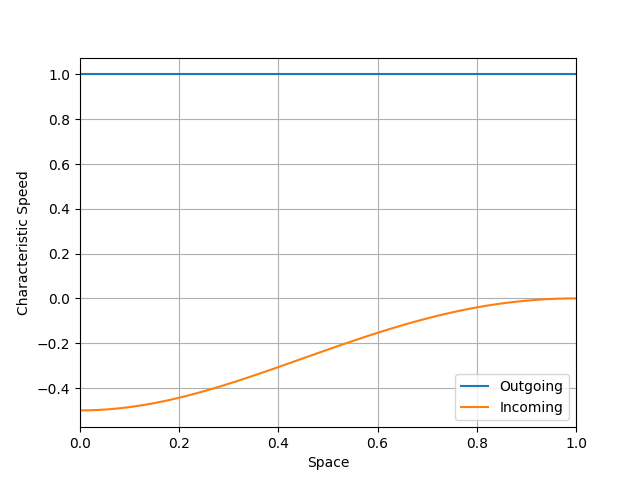
\includegraphics[width=0.5\textwidth]{Images/Good_Speeds.png}
    \caption{Characteristic speeds of the wave equation in hyperboloidal coordinates with $H(R) = \frac{2 R^2 + S^2 - \sqrt{4 R^2 S^2 + S^4}}{2R}$, $\Omega(r) = 1 - \frac{r^2}{S^2}$ and $S = 1$ for outgoing and incoming waves.}
    \label{fig:Good_Speeds}
\end{figure}

Throughout this work, we will sacrifice this very relevant property in exchange for ease of manipulation of the expressions since the goal of this introductory work to the subject is to get accustomed to the coordinate system. The height and compress functions that will used throughout this work are
%
\begin{equation}
    \begin{array}{l c r}
        H(R) = \sqrt{S^2+R^2} & \qquad\qquad\qquad & \Omega(r) = \frac{1}{2} \left(1 - \frac{r^2}{S^2}\right)
    \end{array} \; ,
\end{equation}
%
where $S$ is a constant that determines the size of the compactified domain, which we can choose arbitrarily. To make our domains range from -1 to 1 in the generic case and from 0 to 1 in the spherically symmetric case, we will set $S=1$. As a consequence of our previous choices, we also have
%
\begin{equation}
    \begin{array}{l c r}
        H'(r) = \frac{2 \, r \, S}{S^2 + r^2} & \qquad\qquad\qquad & L(r) = \frac{1}{2} \left(1 + \frac{r^2}{S^2}\right) \; .
    \end{array}
\end{equation}

For this choice of functions, we still have that the incoming light speed decreases as it reaches $\mathscr{I}$. However, we don't have a constant outgoing propagation speed, shown in figure \ref{fig:Bad_Speeds}. The only implication this choice will have in our results is that the wave will take longer to reach $\mathscr{I}$ and will be slightly distorted, which is not problematic since our purpose is to ensure the code converges smoothly toward the solution.

\begin{figure}[h]
    \centering
    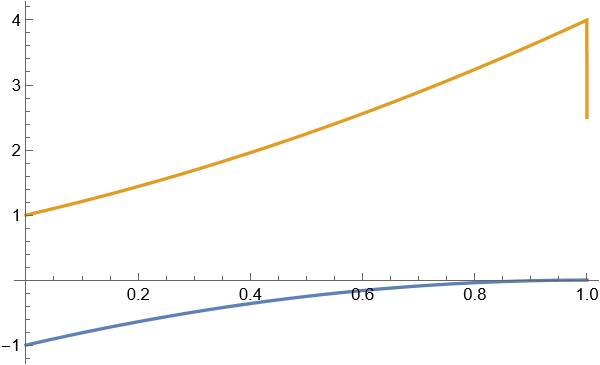
\includegraphics[width=0.5\textwidth]{Images/Bad_Speeds.png}
    \caption{Characteristic speeds of the wave equation in hyperboloidal coordinates with $H(R) = \sqrt{S^2+R^2}$, $\Omega(r) = \frac{1}{2} \left(1 - \frac{r^2}{S^2}\right)$ and $S = 1$ for outgoing and incoming waves.}
    \label{fig:Bad_Speeds}
\end{figure}

\subsection{Computational Setup}

This work is a continuation of my previous work on numerical relativity. As such, the framework used here is the same as the one used there (described in \cite{Ficalho_2023}), with the addition of truncation error matching for the derivatives, interpolation at the boundaries, and the Evans Method for regularization at the origin.

\subsubsection{Truncation Error Matching}

Truncation error matching is a technique used to improve the accuracy of the numerical solution by matching the truncation error of the finite difference scheme used on the boundaries to the truncation error of the one used in the interior of our computational domain. This matching uses a one-sided finite difference scheme on the boundaries such that the leading order error term is the same as the one used in the interior.

In our framework, to approximate the first derivative of a field $\psi$ at an interior point $i$ (writing the leading order error term explicitly), we use 
%
\begin{equation}
    \psi'_i = \frac{\psi_{i+1} - \psi_{i-1}}{2h} - \frac{h^2}{6} \psi'''_i + ...\; ,
\end{equation}
%
where $\psi_{i+1}$ and $\psi_{i-1}$ are the values of the field $\psi$ at the points $i+1$ and $i-1$ respectively, and $h$ is the grid spacing. \cite{Pretorius_2002,Gautam_2021}

To match this leading order term of the error at the left and right boundary points, respectively, we use
%
\begin{equation}
    \psi'_i = \frac{\psi_{i+3} - 4 \psi_{i+2} + 7 \psi_{i+1} - 4 \psi_{i}}{2h} - \frac{h^2}{6} \psi'''_i + ...\;
\end{equation}
%
\begin{equation}
    \psi'_i = \frac{4 \psi_{i} - 7 \psi_{i-1} + 4 \psi_{i-2} - \psi_{i-3}}{2h} - \frac{h^2}{6} \psi'''_i + ...\;
\end{equation}


\subsubsection{Extrapolation at the Boundaries}

Since we are interested in evolving the fields at null infinity, we must choose a boundary condition that allows the fields to propagate out of our computational domain. To do so, we use extrapolation at the outer boundaries of our computational domain to fill the ghost points in those regions. We calculate the value of our fields at the ghost points using
%
\begin{equation}
    \psi_i = 4 \psi_{i-1} - 6 \psi_{i-2} + 4 \psi_{i-3} - \psi_{i-4} \; ,
\end{equation}
%
where $\psi_i$ is the value of the field at the ghost point $i$, and $\psi_{i-1}$, $\psi_{i-2}$, $\psi_{i-3}$ and $\psi_{i-4}$ are the values of the field at the points $i-1$, $i-2$, $i-3$ and $i-4$ respectively.

\subsubsection{Evans Method}
When dealing with operators like the Laplacian in spherical coordinates, we find some formal singularities, like terms where the coefficients are inversely proportional to the radial coordinate, that we must remove for our code to work. To remove those singularities, we can apply the Evans Method. This method involves rewriting the singular terms as a different differential operator, called the Evans operator, which we can evaluate at the grid points. We define this operator as
%
\begin{equation}
    \partial_r \psi + \frac{p}{r}\psi = (p+1) \frac{d(r^p \psi)}{dr^{p+1}}\;,
\end{equation}
%
where $p$ is a constant. This operator can be expressed in terms of the grid points as 
%
\begin{equation}
    (p+1) \frac{d(r^p \psi)}{dr^{p+1}}=(\tilde{D}\psi)_i = (p+1)\frac{r^p_{i+1}\psi_{i+1}-r^p_{i-1}\psi_{i-1}}{r^{p+1}_{i+1}-r^{p+1}_{i-1}}\;,
\end{equation}
%
where the subscripts $i+1$ and $i-1$ denote the grid points $i+1$ and $i-1$ respectively. \cite{Evans_1984}